% Компилировать pdfLaTeX (компилятор Overleaf по умолчанию; задан в latexmkrc).
\documentclass[12pt,a4paper]{article}

\usepackage{iftex}
\ifPDFTeX
  \usepackage[T2A]{fontenc}
  \usepackage[utf8]{inputenc}
\else
  \usepackage{fontspec}
  \setmainfont{CMU Serif}
  \setsansfont{CMU Sans Serif}
  \setmonofont{CMU Typewriter Text}
\fi
\usepackage[english,russian]{babel}
\usepackage{amsmath,amssymb}
\usepackage[left=25mm,right=15mm,top=20mm,bottom=20mm]{geometry}
\usepackage{graphicx}
\usepackage{float}
\usepackage{booktabs}
\usepackage{array}
\usepackage{xcolor}
\usepackage{listings}
\usepackage{caption}
\usepackage{subcaption}
\usepackage{indentfirst}
\usepackage{enumitem}
\usepackage[hidelinks]{hyperref}

\setlength{\parindent}{1.25cm}
\linespread{1.15}
\captionsetup{font=small,labelsep=period}
\setlist{nosep}

\definecolor{codebg}{RGB}{247,247,249}
\definecolor{codekw}{RGB}{0,51,153}
\definecolor{codestr}{RGB}{163,21,21}
\definecolor{codenum}{RGB}{110,110,110}

\lstset{
  language=Python,
  basicstyle=\ttfamily\footnotesize,
  keywordstyle=\color{codekw}\bfseries,
  stringstyle=\color{codestr},
  numberstyle=\tiny\color{codenum},
  backgroundcolor=\color{codebg},
  frame=single,
  rulecolor=\color{black!20},
  breaklines=true,
  breakatwhitespace=false,
  columns=fullflexible,
  keepspaces=true,
  showstringspaces=false,
  tabsize=4,
  upquote=true,
  extendedchars=true
}
\ifPDFTeX
\lstset{literate={А}{{\CYRA}}1 {Б}{{\CYRB}}1 {В}{{\CYRV}}1 {Г}{{\CYRG}}1 {Д}{{\CYRD}}1 {Е}{{\CYRE}}1 {Ё}{{\CYRYO}}1 {Ж}{{\CYRZH}}1 {З}{{\CYRZ}}1 {И}{{\CYRI}}1 {Й}{{\CYRISHRT}}1 {К}{{\CYRK}}1 {Л}{{\CYRL}}1 {М}{{\CYRM}}1 {Н}{{\CYRN}}1 {О}{{\CYRO}}1 {П}{{\CYRP}}1 {Р}{{\CYRR}}1 {С}{{\CYRS}}1 {Т}{{\CYRT}}1 {У}{{\CYRU}}1 {Ф}{{\CYRF}}1 {Х}{{\CYRH}}1 {Ц}{{\CYRC}}1 {Ч}{{\CYRCH}}1 {Ш}{{\CYRSH}}1 {Щ}{{\CYRSHCH}}1 {Ъ}{{\CYRHRDSN}}1 {Ы}{{\CYRERY}}1 {Ь}{{\CYRSFTSN}}1 {Э}{{\CYREREV}}1 {Ю}{{\CYRYU}}1 {Я}{{\CYRYA}}1 {а}{{\cyra}}1 {б}{{\cyrb}}1 {в}{{\cyrv}}1 {г}{{\cyrg}}1 {д}{{\cyrd}}1 {е}{{\cyre}}1 {ё}{{\cyryo}}1 {ж}{{\cyrzh}}1 {з}{{\cyrz}}1 {и}{{\cyri}}1 {й}{{\cyrishrt}}1 {к}{{\cyrk}}1 {л}{{\cyrl}}1 {м}{{\cyrm}}1 {н}{{\cyrn}}1 {о}{{\cyro}}1 {п}{{\cyrp}}1 {р}{{\cyrr}}1 {с}{{\cyrs}}1 {т}{{\cyrt}}1 {у}{{\cyru}}1 {ф}{{\cyrf}}1 {х}{{\cyrh}}1 {ц}{{\cyrc}}1 {ч}{{\cyrch}}1 {ш}{{\cyrsh}}1 {щ}{{\cyrshch}}1 {ъ}{{\cyrhrdsn}}1 {ы}{{\cyrery}}1 {ь}{{\cyrsftsn}}1 {э}{{\cyrerev}}1 {ю}{{\cyryu}}1 {я}{{\cyrya}}1 {°}{{\textdegree}}1}
\fi

\newcommand{\vect}[1]{\mathbf{#1}}
\newcommand{\nrm}{\operatorname{normalize}}

\begin{document}

\begin{titlepage}
\centering
{\small Министерство науки и высшего образования Российской Федерации\\
Федеральное государственное автономное образовательное учреждение высшего образования\\}
\vspace{2mm}
«Национальный исследовательский университет ИТМО»\\
\vspace{2mm}
Факультет программной инженерии и компьютерной техники

\vspace{55mm}
{\Large Лабораторная работа №5}\\[2mm]
по дисциплине «Алгоритмы компьютерной графики»\\[10mm]
{\LARGE\bfseries Формирование изображения\\[2mm] методом трассировки путей}

\vfill
\begin{flushright}
\begin{tabular}{l}
Выполнили:\\
студенты группы P3319\\
Коршун Артем\\
Быков Лев\\[6mm]
Проверил:\\
Жданов Дмитрий Дмитриевич
\end{tabular}
\end{flushright}

\vspace{25mm}
Санкт-Петербург\\
2026
\end{titlepage}

\tableofcontents
\newpage

\section{Задание}

\textbf{Цель работы:} освоить простейшие методы синтеза изображений трёхмерных сцен с учётом локального
освещения методом обратной трассировки лучей; убедиться и доказать корректность сформированного изображения.

\textbf{Задание:} построить изображение трёхмерной сцены с корректным учётом локального освещения методом
обратной трассировки путей (рис.~\ref{fig:task}).

\begin{figure}[H]
\centering
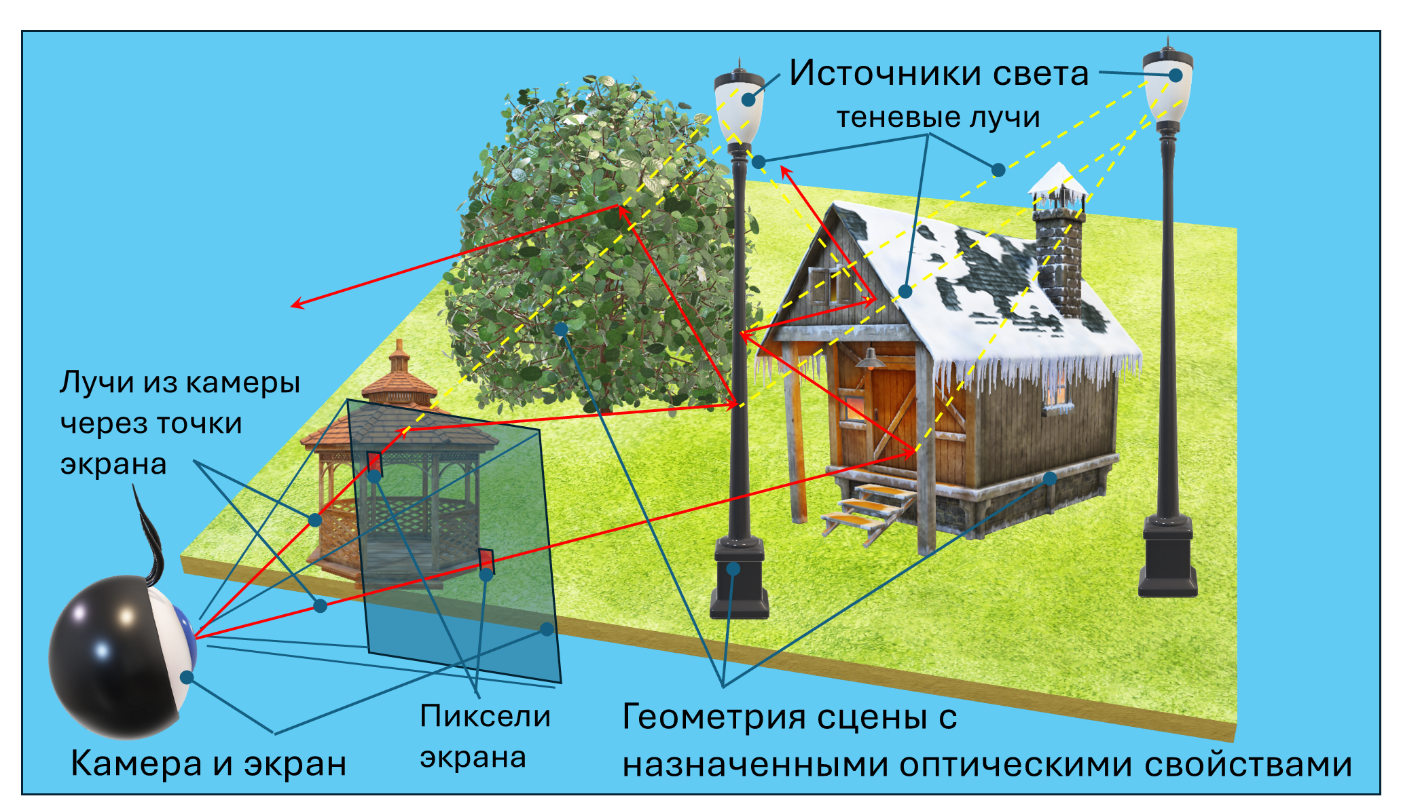
\includegraphics[width=0.85\linewidth]{task_scheme.png}
\caption{Схема обратной трассировки: лучи из камеры через пиксели экрана, теневые лучи к источникам}
\label{fig:task}
\end{figure}

\textbf{Исходные данные и допущения (из задания) и принятые решения:}

\begin{center}
\small
\begin{tabular}{>{\raggedright\arraybackslash}p{0.43\linewidth}>{\raggedright\arraybackslash}p{0.5\linewidth}}
\toprule
Требование & Реализация \\
\midrule
Геометрия — треугольная сетка, вручную или из OBJ & Все объекты — треугольники: прямоугольник, параллелепипед, икосфера, шахматная доска, модель из OBJ-файла (тор-узел, 19\,200 треугольников) \\
Поиск пересечения — своя функция или Embree & Своя функция (Мёллер–Трумбор) + собственная ускоряющая структура BVH (SAH) + готовая библиотека Embree; переключаются параметром \\
Цветовая модель — спектральная или RGB & RGB \\
Ламберт + Фонг / Блинн–Фонг / Кук–Торранс & Ламберт, Фонг и Блинн–Фонг (нормированные формы) \\
Зеркальное отражение и пропускание, $n \ge 1$ & Идеальное зеркальное отражение $k_r$, преломление $k_t$ по закону Снеллиуса с полным внутренним отражением, диффузное пропускание $k_{dt}$ \\
Камера точечная, 500…1000 точек, антиалиасинг & Точечная камера, разрешение задаётся (в работе 600×600, 800×600, 900×500), стратифицированный суперсэмплинг $N$ лучей на пиксель \\
Источники точечные и/или параллельные, диаграмма Ламберта, цветные; корректные тени & Оба типа; точечный — $I(\theta)=I_0\cos\theta$; тени — теневыми лучами \\
Абсолютные яркости $\to$ нормировка $\to$ отсечение $\to$ гамма $\to$ 0…255 $\to$ PPM & Нормировка на максимум, на среднюю яркость 0.5 или на заданное значение; $\gamma = 2.2$; запись PPM (P6) и PNG \\
Простой интерфейс для изменения параметров & Консольный интерфейс (команды \texttt{show/set/render/probe/bench}), сцена в JSON, ввод команд из файла \\
\bottomrule
\end{tabular}
\end{center}

\section{Теоретические сведения}

\subsection{Радиометрические величины}

Свет рассматривается в приближении геометрической оптики как поток частиц, распространяющихся
прямолинейно и независимо. Используются следующие величины:

\begin{itemize}
\item \textbf{поток} $\Phi = dQ/dt$, Вт — энергия, переносимая в единицу времени;
\item \textbf{сила излучения} $I = d\Phi/d\omega$, Вт/ср — поток в единичный телесный угол; ею задаются точечные источники;
\item \textbf{освещённость} $E = d\Phi/dS$, Вт/м$^2$ — поток, падающий на единицу площади;
\item \textbf{яркость} $L = \dfrac{d^2\Phi}{d\omega\, dS\cos\theta}$, Вт/(ср·м$^2$) — величина, которую регистрирует камера; в вакууме не меняется вдоль луча, поэтому изображение — это яркость, пришедшая в камеру по лучу каждого пикселя.
\end{itemize}

\textbf{Точечный источник с диаграммой Ламберта.} Сила излучения зависит от угла $\theta_s$ между осью источника
$\vect a$ и направлением на освещаемую точку: $I(\theta_s) = I_0 \max(0, \cos\theta_s)$.
Освещённость площадки на расстоянии $R$, нормаль которой составляет угол $\theta$ с направлением на источник
(закон обратных квадратов):
\begin{equation}
E = \frac{I(\theta_s)\cos\theta}{R^2}.
\label{eq:point}
\end{equation}

\textbf{Параллельный источник} задаётся освещённостью $E_0$ площадки, перпендикулярной лучам: $E = E_0\cos\theta$.

В программе функция \texttt{light\_sample} для каждой точки возвращает направление на источник $\vect l$,
расстояние $R$ и величину $I(\theta_s)/R^2$ (для параллельного источника — $E_0$); множитель $\cos\theta$
учитывается при расчёте яркости:

\begin{lstlisting}
def light_sample(light, points):
    if light["type"] == "point":
        vec = light["position"] - points
        dist = np.linalg.norm(vec, axis=1)
        to_light = vec / dist[:, None]
        intensity = np.broadcast_to(light["intensity"], points.shape)
        if light["lambert"]:
            intensity = intensity * np.clip(-to_light @ light["axis"], 0.0, None)[:, None]
        return to_light, dist, intensity / (dist ** 2)[:, None]
    to_light = np.broadcast_to(-light["direction"], points.shape)
    return to_light, np.full(len(points), np.inf), np.broadcast_to(light["irradiance"], points.shape)
\end{lstlisting}

\subsection{Уравнение рендеринга и локальное освещение}

Яркость, уходящая из точки $\vect p$ поверхности в направлении $\omega_o$, определяется уравнением рендеринга:
\begin{equation}
L_o(\vect p, \omega_o) = \int_{\Omega} f_r(\vect p, \omega_o, \omega_i)\, L_i(\vect p, \omega_i)\cos\theta_i\, d\omega_i,
\end{equation}
где $f_r$ — двулучевая функция отражательной способности (BRDF), 1/ср.

При \emph{локальном} освещении свет приходит в точку только непосредственно от точечных и параллельных
источников и по идеальным зеркальным направлениям. Интеграл превращается в сумму:
\begin{equation}
L_o(\vect p, \omega_o) = \sum_{j} f(\omega_j, \omega_o)\, E_j\, V_j \;+\; k_r L(\vect p, \omega_r) \;+\; k_t L(\vect p, \omega_t),
\label{eq:local}
\end{equation}
где $E_j$ — освещённость от $j$-го источника по формуле~(\ref{eq:point}) без косинуса, умноженная на $\cos\theta_j$;
$V_j\in\{0,1\}$ — видимость источника (0 — точка в тени); $\omega_r$, $\omega_t$ — направления зеркально отражённого
и преломлённого лучей; $k_r$, $k_t$ — коэффициенты зеркального отражения и пропускания. Слагаемые
$L(\vect p,\omega_r)$ и $L(\vect p,\omega_t)$ вычисляются рекурсивно трассировкой вторичных лучей.

\subsection{Модели отражения}

\textbf{Модель Ламберта} (идеальное диффузное отражение): $f_d = k_d/\pi$. Деление на $\pi$ обеспечивает
закон сохранения энергии: при $k_d=1$ светимость поверхности $M = \pi L = E$.

\textbf{Модель Фонга} (нормированная): блик вокруг зеркально отражённого направления на источник
$\vect r = 2(\vect n\cdot\vect l)\vect n - \vect l$:
\begin{equation}
f_s^{\text{Phong}} = k_s\,\frac{n+2}{2\pi}\,\max(0, \vect r\cdot\vect v)^{n}.
\end{equation}

\textbf{Модель Блинна–Фонга} (нормированная): вместо отражённого вектора используется полувектор
$\vect h = \nrm(\vect l + \vect v)$:
\begin{equation}
f_s^{\text{Blinn}} = k_s\,\frac{n+8}{8\pi}\,\max(0, \vect n\cdot\vect h)^{n}.
\end{equation}

Здесь $\vect n$ — нормаль, $\vect l$ — направление на источник, $\vect v$ — направление на наблюдателя,
$n$ — показатель блеска. Нормировочные множители сохраняют отражённую энергию при изменении $n$.
Модель выбирается для каждого материала (\texttt{"model": "phong"} или \texttt{"blinn"}):

\begin{lstlisting}
def brdf_specular(scene, mat, normal, to_light, view):
    ks = scene.ks[mat]
    n = scene.shininess[mat]
    blinn = scene.blinn[mat]
    half = normalize(to_light + view)
    cos_h = np.clip(dot(normal, half), 0.0, 1.0)
    mirror = 2.0 * dot(normal, to_light)[:, None] * normal - to_light
    cos_r = np.clip(dot(mirror, view), 0.0, 1.0)
    blinn_value = (n + 8.0) / (8.0 * np.pi) * cos_h ** n
    phong_value = (n + 2.0) / (2.0 * np.pi) * cos_r ** n
    return ks * np.where(blinn, blinn_value, phong_value)[:, None]
\end{lstlisting}

\textbf{Диффузное пропускание.} Если источник находится с обратной стороны поверхности, вклад вычисляется по
Ламберту с коэффициентом $k_{dt}$: $f_{dt} = k_{dt}/\pi$ (полупрозрачная бумага, абажур).

Для каждого источника вклад в яркость точки (формула~(\ref{eq:local})):
\begin{equation}
L_j = \begin{cases}
\left(\dfrac{k_d}{\pi} + f_s\right)\dfrac{I(\theta_s)}{R^2}\max(0,\cos\theta)\,V_j, & \text{источник со стороны наблюдателя},\\[3mm]
\dfrac{k_{dt}}{\pi}\dfrac{I(\theta_s)}{R^2}\max(0,-\cos\theta)\,V_j, & \text{источник с обратной стороны}.
\end{cases}
\end{equation}

\begin{lstlisting}
reflected = (kd[idx] / np.pi + brdf_specular(scene, mat[idx], nsf[idx], to_light[idx], view[idx])) * np.clip(c, 0.0, None)[:, None]
transmitted = kdt[idx] / np.pi * np.clip(-c, 0.0, None)[:, None]
radiance[idx] += np.where(f[:, None], reflected, transmitted) * irradiance[idx]
\end{lstlisting}

Закон сохранения энергии требует для каждого канала $k_d + k_s + k_r + k_t + k_{dt} \le 1$; это проверяется
для всех материалов сцен (раздел~\ref{sec:verify}).

\subsection{Зеркальное отражение и преломление}

Направление идеально отражённого луча (угол падения равен углу отражения):
\begin{equation}
\vect d_r = \vect d - 2(\vect d\cdot\vect n)\,\vect n.
\end{equation}

Направление преломлённого луча по закону Снеллиуса $n_1\sin\theta_1 = n_2\sin\theta_2$; при $\eta = n_1/n_2$ и
$\cos\theta_1 = -\vect d\cdot\vect n$ ($\vect n$ направлена навстречу лучу):
\begin{equation}
k = 1 - \eta^2(1-\cos^2\theta_1),\qquad
\vect d_t = \eta\,\vect d + \left(\eta\cos\theta_1 - \sqrt{k}\right)\vect n.
\end{equation}
Если $k<0$, преломлённого луча нет — \textbf{полное внутреннее отражение}; тогда коэффициент $k_t$ добавляется к
$k_r$. Луч входит в тело, если $\vect d\cdot\vect n_g < 0$ ($\eta = 1/n$), иначе выходит ($\eta = n$).
Среда снаружи — воздух ($n=1$), внутри тела — однородная прозрачная среда с постоянным $n\ge1$.

\begin{lstlisting}
def refract(dirs, normal, eta):
    cos_i = -dot(dirs, normal)
    k = 1.0 - eta ** 2 * (1.0 - cos_i ** 2)
    tir = k < 0.0
    out = eta[:, None] * dirs + (eta * cos_i - np.sqrt(np.clip(k, 0.0, None)))[:, None] * normal
    return normalize(out), tir


def reflect(dirs, normal):
    return dirs - 2.0 * dot(dirs, normal)[:, None] * normal
\end{lstlisting}

\subsection{Обратная трассировка путей}

При \emph{обратной} трассировке лучи выпускаются не из источников, а из камеры через пиксели экрана: в камеру
попадает только свет, пришедший по этим лучам (закон обратимости световых лучей). Для каждого луча:

\begin{enumerate}
\item находится ближайшее пересечение со сценой (если его нет — яркость фона);
\item в точке пересечения вычисляется прямое освещение от всех источников; видимость $V_j$ определяется
      \textbf{теневым лучом} от точки к источнику;
\item порождаются вторичные лучи — отражённый с весом $k_r$ и преломлённый с весом $k_t$; их яркость добавляется
      к пикселю с весом, равным произведению коэффициентов вдоль пути;
\item рекурсия ограничена глубиной \texttt{max\_depth} и минимальным весом луча ($10^{-4}$).
\end{enumerate}

Цепочка отрезков от камеры через точки отражений/преломлений образует \textbf{путь}. Реализовано два режима:

\begin{itemize}
\item \texttt{split} — в каждой точке путь разветвляется на отражённый и преломлённый (классическая схема Уиттеда);
\item \texttt{path} — в каждой точке случайно выбирается одно продолжение (метод Монте-Карло, «русская рулетка»):
      отражение с вероятностью $p_r$, преломление с $p_t$, обрыв с $1-p_r-p_t$, где
      $p_r = \bar k_r / \max(1, \bar k_r + \bar k_t)$, $p_t = \bar k_t / \max(1, \bar k_r + \bar k_t)$
      ($\bar k$ — среднее по каналам). Вес продолжения делится на вероятность: $w' = w\,k_r/p_r$, поэтому
      математическое ожидание совпадает с режимом \texttt{split}, а число лучей не растёт.
\end{itemize}

Все лучи одного «поколения» обрабатываются вместе (массивами \texttt{numpy}); вклад луча прибавляется к его
пикселю по индексу \texttt{idx}:

\begin{lstlisting}
for depth in range(settings["max_depth"] + 1):
    if len(idx) == 0:
        break
    t, tid, u, v = backend.intersect(orig, dirs)
    stats["rays"] += len(idx)
    miss = tid < 0
    accumulate(result, idx[miss], weight[miss] * background)
    hit = ~miss
    orig, dirs, t, tid, u, v, idx, weight = orig[hit], dirs[hit], t[hit], tid[hit], u[hit], v[hit], idx[hit], weight[hit]
    points, ngf, nsf, mat, entering = surface(scene, orig, dirs, t, tid, u, v)
    local = direct_light(scene, backend, points, ngf, nsf, -dirs, mat, stats)
    accumulate(result, idx, weight * local)
    if depth == settings["max_depth"]:
        break
    eta = np.where(entering, 1.0 / scene.ior[mat], scene.ior[mat])
    refr_dirs, tir = refract(dirs, nsf, eta)
    kt = np.where(tir[:, None], 0.0, scene.kt[mat])
    kr = scene.kr[mat] + np.where(tir[:, None], scene.kt[mat], 0.0)
    refl_dirs = reflect(dirs, nsf)
\end{lstlisting}

Выбор продолжения в режиме \texttt{path}:

\begin{lstlisting}
pr = kr.mean(axis=1)
pt = kt.mean(axis=1)
total = np.maximum(pr + pt, 1.0)
pr, pt = pr / total, pt / total
x = rng.random(len(idx))
take_r = x < pr
take_t = (x >= pr) & (x < pr + pt)
wr = kr / np.where(pr > 0.0, pr, 1.0)[:, None]
wt = kt / np.where(pt > 0.0, pt, 1.0)[:, None]
\end{lstlisting}

\section{Реализация}

\subsection{Структура программы}

Программа написана на Python~3 с использованием \texttt{numpy} (векторные вычисления), \texttt{numba}
(JIT-компиляция и многопоточность для поиска пересечений), \texttt{embreex} (обёртка Intel Embree) и \texttt{Pillow}
(сохранение PNG).

\begin{center}
\small
\begin{tabular}{>{\ttfamily}l>{\raggedright\arraybackslash}p{0.72\linewidth}}
\toprule
\normalfont Файл & Назначение \\
\midrule
main.py & консольный интерфейс, параметры командной строки, ввод команд из файла \\
scene.py & чтение сцены (JSON), построение треугольной сетки, загрузка OBJ, материалы, источники \\
accel.py & пересечение луч–треугольник, построение и обход BVH, полный перебор, обёртка Embree \\
render.py & камера, антиалиасинг, освещение, тени, отражение, преломление, нормировка, гамма, PPM \\
verify.py & доказательство корректности \\
experiments.py & построение иллюстраций и замеры производительности для отчёта \\
make\_models.py & генерация OBJ-модели тор-узла \\
scenes/*.json & сцены: \texttt{room}, \texttt{outdoor}, \texttt{materials}, \texttt{test\_plane}, \texttt{test\_shadow} \\
\bottomrule
\end{tabular}
\end{center}

\subsection{Сцена и треугольная сетка}

Сцена описывается JSON-файлом: камера, параметры рендера, материалы, объекты, источники. Пример фрагмента:

\begin{lstlisting}[language={}]
"materials": {
  "glass":   {"ks": [0.05,0.05,0.05], "shininess": 400, "kr": [0.07,0.07,0.07], "kt": [0.88,0.88,0.88], "ior": 1.5},
  "plastic": {"kd": [0.08,0.2,0.65], "ks": [0.35,0.35,0.35], "shininess": 60, "model": "blinn"}
},
"objects": [
  {"type": "sphere", "radius": 0.32, "subdiv": 4, "position": [-0.2,0.32,0.45], "smooth": true, "material": "glass"},
  {"type": "obj", "file": "../models/knot.obj", "scale": 0.24, "position": [0.45,0.42,-0.2],
   "rotate": [70,0,15], "smooth": true, "material": "plastic"}
],
"lights": [
  {"type": "point", "position": [0,1.96,0.2], "direction": [0,-1,0], "intensity": [3.0,2.8,2.5], "lambert": true}
]
\end{lstlisting}

Каждый объект превращается в треугольники: прямоугольник (2), параллелепипед (12), икосфера (икосаэдр,
каждый треугольник которого $s$ раз делится на 4 с проецированием новых вершин на сферу: $20\cdot4^s$
треугольников), шахматная доска, модель из OBJ-файла. Затем применяются масштаб, поворот (углы Эйлера) и перенос.
Чтение OBJ: строки \texttt{v} — вершины, строки \texttt{f} — грани (многоугольники разбиваются веером на треугольники):

\begin{lstlisting}
def load_obj(path):
    verts = []
    faces = []
    with open(path, encoding="utf-8") as f:
        for line in f:
            parts = line.split()
            if not parts:
                continue
            if parts[0] == "v":
                verts.append([float(x) for x in parts[1:4]])
            elif parts[0] == "f":
                idx = []
                for token in parts[1:]:
                    k = int(token.split("/")[0])
                    idx.append(k - 1 if k > 0 else len(verts) + k)
                for k in range(1, len(idx) - 1):
                    faces.append([idx[0], idx[k], idx[k + 1]])
    return np.array(verts, dtype=np.float64), np.array(faces)
\end{lstlisting}

Для гладких объектов (\texttt{"smooth": true}) в вершинах вычисляются усреднённые нормали соседних граней, а в точке
попадания с барицентрическими координатами $(u,v)$ нормаль интерполируется:
$\vect n_s = \nrm\big((1-u-v)\vect n_0 + u\vect n_1 + v\vect n_2\big)$. Для смещения начала вторичных лучей
используется геометрическая нормаль грани $\vect n_g$. Обе нормали разворачиваются навстречу лучу (поверхности двусторонние):

\begin{lstlisting}
def surface(scene, orig, dirs, t, tid, u, v):
    points = orig + t[:, None] * dirs
    ng = scene.face_normals[tid]
    vn = scene.vertex_normals[tid]
    w = 1.0 - u - v
    ns = normalize(w[:, None] * vn[:, 0] + u[:, None] * vn[:, 1] + v[:, None] * vn[:, 2])
    side = np.where(dot(dirs, ng) < 0.0, 1.0, -1.0)
    ngf = ng * side[:, None]
    nsf = ns * side[:, None]
    bad = dot(nsf, ngf) <= 0.0
    nsf[bad] = ngf[bad]
    return points, ngf, nsf, scene.tri_material[tid], side > 0.0
\end{lstlisting}

\subsection{Камера, первичные лучи и антиалиасинг}

Камера точечная: положение $\vect c$, точка взгляда $\vect t$, вектор «вверх» $\vect{up}$, вертикальный угол обзора $\varphi$,
разрешение $W\times H$. Базис камеры:
\begin{equation}
\vect f = \nrm(\vect t - \vect c),\quad \vect r = \nrm(\vect f\times\vect{up}),\quad \vect u = \vect r\times\vect f.
\end{equation}
Луч через точку экрана $(p_x, p_y)$ (в пикселях):
\begin{equation}
x = \left(\frac{2p_x}{W}-1\right)\tan\frac{\varphi}{2}\,\frac{W}{H},\quad
y = \left(1-\frac{2p_y}{H}\right)\tan\frac{\varphi}{2},\quad
\vect d = \nrm(\vect f + x\,\vect r + y\,\vect u).
\end{equation}

\begin{lstlisting}
def primary_rays(cam, px, py):
    width, height = cam["width"], cam["height"]
    pos, forward, right, up = camera_basis(cam)
    tan = np.tan(np.radians(cam["fov"]) / 2.0)
    x = (2.0 * px / width - 1.0) * tan * width / height
    y = (1.0 - 2.0 * py / height) * tan
    dirs = normalize(forward + x[:, None] * right + y[:, None] * up)
    return np.broadcast_to(pos, dirs.shape).copy(), dirs
\end{lstlisting}

\textbf{Антиалиасинг.} Пиксель $(i,j)$ делится на $k\times k$ подклеток ($N=k^2$ лучей на пиксель, \texttt{spp});
в подклетке $s$ берётся случайная точка (стратифицированный джиттер), яркость пикселя — среднее:
\begin{equation}
p_x = j + \frac{(s \bmod k) + \xi_1}{k},\quad p_y = i + \frac{\lfloor s/k\rfloor + \xi_2}{k},\quad
L_{ij} = \frac{1}{N}\sum_{s=0}^{N-1} L(\vect c, \vect d_s),\qquad \xi_{1,2}\in[0,1).
\end{equation}

\begin{lstlisting}
def pixel_offsets(spp, index, count, rng):
    if spp == 1:
        return np.full(count, 0.5), np.full(count, 0.5)
    k = int(round(np.sqrt(spp)))
    if k * k == spp:
        return (index % k + rng.random(count)) / k, (index // k + rng.random(count)) / k
    return rng.random(count), rng.random(count)
\end{lstlisting}

\subsection{Пересечение луча с треугольником}

Используется алгоритм Мёллера–Трумбора. Точка луча $\vect o + t\vect d$ и точка треугольника в барицентрических
координатах $\vect v_0 + u\vect e_1 + v\vect e_2$ ($\vect e_1 = \vect v_1-\vect v_0$, $\vect e_2 = \vect v_2-\vect v_0$)
совпадают, если $[-\vect d,\ \vect e_1,\ \vect e_2](t,u,v)^T = \vect o-\vect v_0$. По правилу Крамера при
$\vect s = \vect o-\vect v_0$, $\vect P = \vect d\times\vect e_2$, $\vect Q = \vect s\times\vect e_1$:
\begin{equation}
\det = \vect e_1\cdot\vect P,\quad u = \frac{\vect s\cdot\vect P}{\det},\quad v = \frac{\vect d\cdot\vect Q}{\det},\quad t = \frac{\vect e_2\cdot\vect Q}{\det}.
\end{equation}
Пересечение есть, если $\det\ne0$, $u\ge0$, $v\ge0$, $u+v\le1$ и $0<t<t_{\max}$. Функция компилируется \texttt{numba}:

\begin{lstlisting}
@njit(cache=True, inline="always")
def ray_triangle(ox, oy, oz, dx, dy, dz, v0, e1, e2, j, tmax):
    px = dy * e2[j, 2] - dz * e2[j, 1]
    py = dz * e2[j, 0] - dx * e2[j, 2]
    pz = dx * e2[j, 1] - dy * e2[j, 0]
    det = e1[j, 0] * px + e1[j, 1] * py + e1[j, 2] * pz
    if abs(det) < 1e-14:
        return -1.0, 0.0, 0.0
    inv = 1.0 / det
    sx = ox - v0[j, 0]
    sy = oy - v0[j, 1]
    sz = oz - v0[j, 2]
    u = (sx * px + sy * py + sz * pz) * inv
    if u < 0.0 or u > 1.0:
        return -1.0, 0.0, 0.0
    qx = sy * e1[j, 2] - sz * e1[j, 1]
    qy = sz * e1[j, 0] - sx * e1[j, 2]
    qz = sx * e1[j, 1] - sy * e1[j, 0]
    v = (dx * qx + dy * qy + dz * qz) * inv
    if v < 0.0 or u + v > 1.0:
        return -1.0, 0.0, 0.0
    t = (e2[j, 0] * qx + e2[j, 1] * qy + e2[j, 2] * qz) * inv
    if t <= T_EPS or t >= tmax:
        return -1.0, 0.0, 0.0
    return t, u, v
\end{lstlisting}

Полный перебор (\texttt{brute}) проверяет все $N$ треугольников для каждого луча — сложность $O(N)$ на луч.
Он используется как эталон.

\subsection{Ускоряющая структура BVH}

\textbf{Иерархия ограничивающих объёмов} (Bounding Volume Hierarchy) — двоичное дерево, каждый узел которого хранит
ограничивающий параллелепипед со сторонами вдоль осей (AABB) для своей группы треугольников; в листьях хранятся
сами треугольники (не более 16). Если луч не пересекает параллелепипед узла, всё его поддерево пропускается, поэтому
число проверок на луч в среднем растёт как $O(\log N)$.

\textbf{Пересечение луча с AABB} (slab-тест). Для каждой оси находятся параметры входа и выхода из слоя между
двумя плоскостями, затем пересекаются интервалы:
\begin{equation}
t_{1,2}^{(a)} = \frac{b^{(a)}_{\min,\max} - o^{(a)}}{d^{(a)}},\quad
t_n = \max_a \min(t_1^{(a)}, t_2^{(a)}),\quad t_f = \min_a \max(t_1^{(a)}, t_2^{(a)});
\end{equation}
луч пересекает параллелепипед, если $t_n\le t_f$, $t_f\ge0$ и $t_n < t_{\text{best}}$ (ближе уже найденного пересечения).

\begin{lstlisting}
@njit(cache=True, inline="always")
def ray_box(ox, oy, oz, ix, iy, iz, bmin, bmax, node, tmax):
    t1 = (bmin[node, 0] - ox) * ix
    t2 = (bmax[node, 0] - ox) * ix
    tn = min(t1, t2)
    tf = max(t1, t2)
    t1 = (bmin[node, 1] - oy) * iy
    t2 = (bmax[node, 1] - oy) * iy
    tn = max(tn, min(t1, t2))
    tf = min(tf, max(t1, t2))
    t1 = (bmin[node, 2] - oz) * iz
    t2 = (bmax[node, 2] - oz) * iz
    tn = max(tn, min(t1, t2))
    tf = min(tf, max(t1, t2))
    if tn <= tf and tf >= 0.0 and tn < tmax:
        return tn
    return np.inf
\end{lstlisting}

\textbf{Построение по эвристике площади поверхности (SAH).} Вероятность попадания случайного луча в выпуклое тело,
находящееся внутри другого, пропорциональна отношению площадей их поверхностей. Поэтому ожидаемая стоимость
разбиения узла с площадью $S$ на детей с $N_L$, $N_R$ треугольниками и площадями $S_L$, $S_R$:
\begin{equation}
C = C_{\text{trav}} + \frac{S_L}{S} N_L C_{\text{tri}} + \frac{S_R}{S} N_R C_{\text{tri}},\qquad C_{\text{trav}} = C_{\text{tri}} = 1.
\end{equation}
Для каждой оси треугольники сортируются по центрам ограничивающих параллелепипедов; накопленные минимумы и максимумы
(префиксные и суффиксные) дают $S_L$ и $S_R$ для всех $N-1$ разрезов сразу. Выбирается разрез с минимальной $C$.
Если $C\ge N$ (делить невыгодно) и $N\le16$, или $N\le4$, узел становится листом:

\begin{lstlisting}
for axis in range(3):
    srt = idx[np.argsort(cent[idx, axis], kind="stable")]
    lmin = np.minimum.accumulate(tmin[srt], axis=0)[:-1]
    lmax = np.maximum.accumulate(tmax[srt], axis=0)[:-1]
    rmin = np.minimum.accumulate(tmin[srt][::-1], axis=0)[::-1][1:]
    rmax = np.maximum.accumulate(tmax[srt][::-1], axis=0)[::-1][1:]
    cost = 1.0 + (surface_area(lmin, lmax) * k + surface_area(rmin, rmax) * (m - k)) / area
    i = int(np.argmin(cost))
    if cost[i] < best_cost:
        best_cost, best_split, best_order = cost[i], i + 1, srt
if best_order is None or (best_cost >= m and m <= max_leaf):
    start[node], count[node] = s, m
    continue
\end{lstlisting}

Дерево хранится в плоских массивах (\texttt{bmin}, \texttt{bmax}, \texttt{left}, \texttt{right}, \texttt{start},
\texttt{count}), треугольники переупорядочиваются так, чтобы треугольники каждого листа шли подряд.

\textbf{Обход.} Используется стек узлов. Узел, расстояние до параллелепипеда которого больше уже найденного
пересечения, пропускается. Для внутреннего узла проверяются оба ребёнка и в стек кладутся пересечённые, ближний —
последним, чтобы он обрабатывался первым и быстрее сокращал $t_{\text{best}}$. Лучи распределяются по потокам (\texttt{prange}):

\begin{lstlisting}
while sp > 0:
    sp -= 1
    node = stack[sp]
    if dist[sp] >= best:
        continue
    steps += 1
    if count[node] > 0:
        for j in range(start[node], start[node] + count[node]):
            t, u, v = ray_triangle(ox, oy, oz, dx, dy, dz, v0, e1, e2, j, best)
            if t > 0.0:
                best, hit, bu, bv = t, j, u, v
    else:
        l = left[node]
        r = right[node]
        tl = ray_box(ox, oy, oz, ix, iy, iz, bmin, bmax, l, best)
        tr = ray_box(ox, oy, oz, ix, iy, iz, bmin, bmax, r, best)
        hl = tl < np.inf
        hr = tr < np.inf
        if hl and hr:
            if tl <= tr:
                stack[sp] = r
                dist[sp] = tr
                stack[sp + 1] = l
                dist[sp + 1] = tl
            else:
                stack[sp] = l
                dist[sp] = tl
                stack[sp + 1] = r
                dist[sp + 1] = tr
            sp += 2
        elif hl:
            stack[sp] = l
            dist[sp] = tl
            sp += 1
        elif hr:
            stack[sp] = r
            dist[sp] = tr
            sp += 1
\end{lstlisting}

Для теневых лучей используется отдельная функция \texttt{bvh\_occluded}: достаточно найти \emph{любое} пересечение
с $t < R$, после чего обход прекращается.

На рис.~\ref{fig:bvh} показаны параллелепипеды узлов BVH уровней 1–4 для сцены «комната» и число узлов,
посещённых первичным лучом каждого пикселя. Для 24\,342 треугольников дерево содержит 15\,117 узлов (7\,559 листьев,
глубина 17); первичный луч посещает в среднем 9.9 узла (максимум 80) — вместо проверки всех 24\,342 треугольников.

\begin{figure}[H]
\centering
\begin{subfigure}{0.48\linewidth}\centering
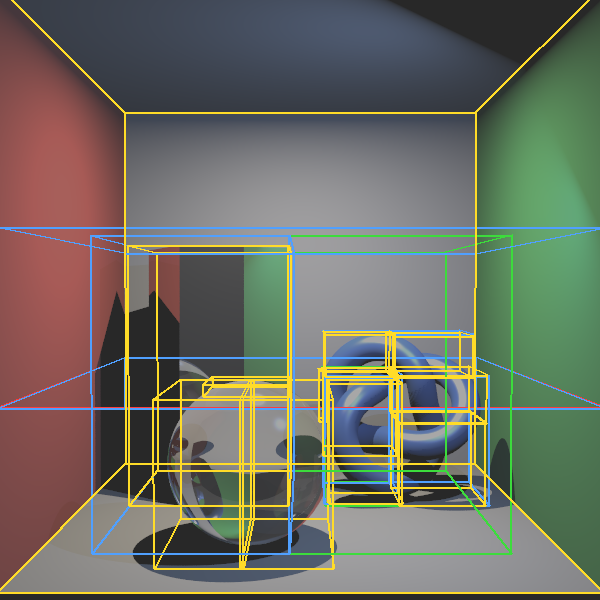
\includegraphics[width=\linewidth]{bvh_boxes.png}
\caption{узлы уровней 1 (красный), 2 (зелёный), 3 (синий), 4 (жёлтый)}
\end{subfigure}\hfill
\begin{subfigure}{0.48\linewidth}\centering
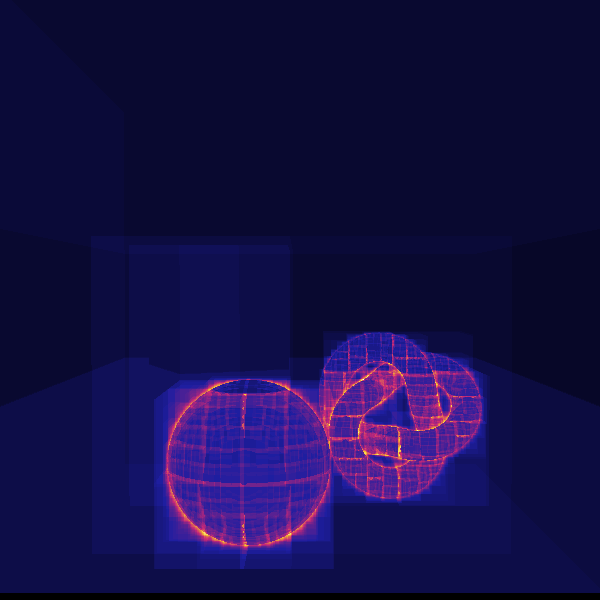
\includegraphics[width=\linewidth]{bvh_heatmap.png}
\caption{число посещённых узлов на первичный луч (тёмный — мало, светлый — до 80)}
\end{subfigure}
\caption{Ускоряющая структура BVH сцены «комната»}
\label{fig:bvh}
\end{figure}

\subsection{Готовая библиотека трассировки Embree}

Intel Embree — библиотека высокопроизводительных ядер трассировки лучей (BVH с SIMD-оптимизацией обхода).
Из Python она используется через пакет \texttt{embreex}: массив треугольников передаётся в сцену Embree, метод
\texttt{run} возвращает для каждого луча расстояние \texttt{tfar}, номер треугольника \texttt{primID} и барицентрические
координаты $u, v$ (в той же параметризации, что и у Мёллера–Трумбора); запрос \texttt{OCCLUDED} — проверка тени.
Все три способа поиска пересечений имеют одинаковый интерфейс и переключаются параметром \texttt{render.backend}
(\texttt{brute}, \texttt{bvh}, \texttt{embree}).

\begin{lstlisting}
class EmbreeBackend:
    name = "embree"

    def __init__(self, triangles):
        from embreex import rtcore_scene
        from embreex.mesh_construction import TriangleMesh
        start_time = time.perf_counter()
        self.scene = rtcore_scene.EmbreeScene()
        self.mesh = TriangleMesh(self.scene, triangles.astype(np.float32))
        self.scene.run(np.zeros((1, 3), np.float32), np.ones((1, 3), np.float32))
        self.build_time = time.perf_counter() - start_time

    def intersect(self, orig, dirs, tfar=None):
        orig, dirs, tfar = as_rays(orig, dirs, tfar)
        res = self.scene.run(orig.astype(np.float32), dirs.astype(np.float32),
                             dists=np.minimum(tfar, 1e30).astype(np.float32), output=1)
        tid = res["primID"].astype(np.int64)
        t = res["tfar"].astype(np.float64)
        t[tid < 0] = np.inf
        return t, tid, res["u"].astype(np.float64), res["v"].astype(np.float64)

    def occluded(self, orig, dirs, tfar):
        orig, dirs, tfar = as_rays(orig, dirs, tfar)
        res = self.scene.run(orig.astype(np.float32), dirs.astype(np.float32),
                             dists=np.minimum(tfar, 1e30).astype(np.float32), query="OCCLUDED")
        return res >= 0
\end{lstlisting}

\subsection{Тени}

Для каждой освещаемой точки и каждого источника строится теневой луч из точки $\vect p + \varepsilon\vect n_g$
к источнику с $t_{\max} = R - 2\varepsilon$ ($\varepsilon = 10^{-4}\cdot$размер сцены). Сдвиг начала по
геометрической нормали исключает ложное самозатенение из-за погрешности вычислений. Если луч перекрыт, $V_j=0$.
Теневые лучи строятся только для точек, где вклад источника может быть ненулевым:

\begin{lstlisting}
for light in scene.lights:
    to_light, dist, irradiance = light_sample(light, points)
    cos_n = dot(nsf, to_light)
    front = dot(ngf, to_light) > 0.0
    active = (irradiance.max(axis=1) > 0.0) & np.where(front, reflective, transmissive)
    if not active.any():
        continue
    idx = np.nonzero(active)[0]
    offset = np.where(front[idx], scene.eps, -scene.eps)[:, None] * ngf[idx]
    blocked = backend.occluded(points[idx] + offset, to_light[idx], dist[idx] - 2.0 * scene.eps)
    stats["shadow_rays"] += len(idx)
    idx = idx[~blocked]
\end{lstlisting}

Прозрачные тела для теневых лучей непрозрачны: при обратной трассировке путь «точка — преломляющая поверхность —
точечный источник» найти невозможно (каустики требуют прямой трассировки), поэтому в модели локального освещения
это корректное поведение.

\subsection{Перевод в относительные яркости, гамма-коррекция, PPM}

Трассировка даёт изображение в абсолютных яркостях $L$, Вт/(ср·м$^2$). Перевод в отображаемые значения:
\begin{equation}
V_{\text{rel}} = \min\!\left(1, \frac{L}{L_{\text{norm}}}\right),\qquad V_{\text{corr}} = V_{\text{rel}}^{1/\gamma},\ \gamma = 2.2,
\qquad V_{255} = \operatorname{round}(255\,V_{\text{corr}}),
\end{equation}
где нормировочное значение $L_{\text{norm}}$ выбирается одним из способов: \texttt{max} — максимальная яркость
изображения; \texttt{mean} — так, чтобы средняя яркость $Y = 0.2126R + 0.7152G + 0.0722B$ стала равна 0.5
($L_{\text{norm}} = \bar Y/0.5$); \texttt{fixed} — заранее заданное значение. Всё, что больше 1, отсекается.

\begin{lstlisting}
def normalization(image, mode, value):
    if mode == "max":
        return float(image.max())
    if mode == "mean":
        return float(luminance(image).mean() / 0.5)
    return float(value)


def tone_map(image, mode="mean", value=1.0, gamma=2.2):
    norm = normalization(image, mode, value)
    relative = np.clip(image / norm, 0.0, 1.0)
    return np.round(relative ** (1.0 / gamma) * 255.0).astype(np.uint8), norm


def save_ppm(path, image8):
    height, width = image8.shape[:2]
    with open(path, "wb") as f:
        f.write(b"P6\n%d %d\n255\n" % (width, height))
        f.write(np.ascontiguousarray(image8).tobytes())
\end{lstlisting}

Формат PPM (P6): текстовый заголовок «\texttt{P6}, ширина, высота, 255», затем байты $R, G, B$ всех пикселей построчно.
Дополнительно сохраняются PNG и массив абсолютных яркостей (\texttt{.npy}).

\subsection{Интерфейс}

\begin{sloppypar}
Программа запускается командой \texttt{python main.py scenes/room.json}. В интерактивном режиме доступны команды:
\texttt{show [раздел]} — показать параметры; \texttt{set путь значение} — изменить любой параметр сцены (значение в
формате JSON); \texttt{render} — построить изображение; \texttt{probe x y} — вывести абсолютную яркость в пикселе;
\texttt{bench N} — сравнить способы поиска пересечений; \texttt{save}/\texttt{load} — сохранить/загрузить сцену.
Параметры можно задать и в командной строке (\texttt{--set render.spp=4 --render}), а последовательность команд —
прочитать из файла (\texttt{--commands tests/demo\_commands.txt}). Фрагмент сеанса из файла с тестовыми данными:
\end{sloppypar}

\begin{lstlisting}[language={}]
lab5> set render.spp 4
lab5> render
Ускоряющая структура embree построена за 0.040 с
Рендер 500x500, 4 лучей на пиксель, глубина 6, режим split, 24342 triangles, 7 materials, 2 lights
Время 2.77 с, лучей 1734791, теневых лучей 2661513 (1.59 млн лучей/с)
Яркость: макс 1.315, средняя 0.05909, нормировка на 0.2 (fixed), гамма 2.20
lab5> probe 250 420
Яркость L(250, 420) = [0.015362, 0.0154428, 0.0165278] Вт/(ср*м2)
lab5> set lights.0.position [-0.5,1.9,0.5]
lab5> set lights.0.intensity [4,2,1]
lab5> set materials.glass.ior 1.33
lab5> set materials.plastic.model "phong"
lab5> set render.backend "bvh"
lab5> render
Ускоряющая структура bvh построена за 0.979 с
\end{lstlisting}

\begin{figure}[H]
\centering
\begin{subfigure}{0.42\linewidth}\centering
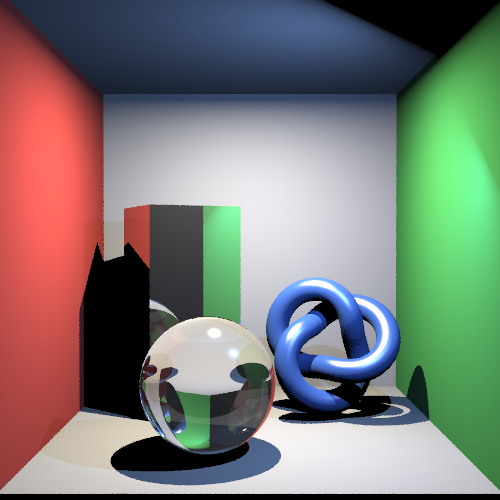
\includegraphics[width=\linewidth]{demo_base.png}
\caption{исходная сцена (Embree)}
\end{subfigure}\hspace{6mm}
\begin{subfigure}{0.42\linewidth}\centering
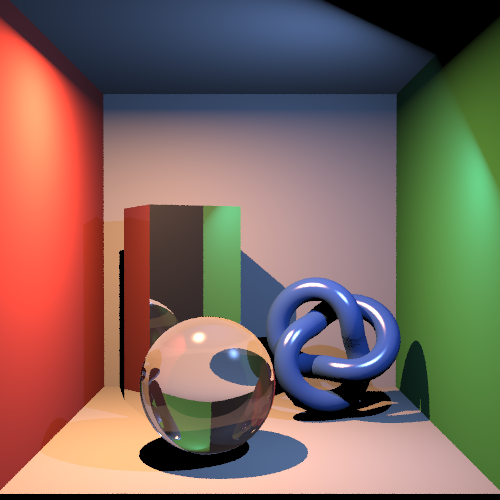
\includegraphics[width=\linewidth]{demo_changed.png}
\caption{источник сдвинут и окрашен, $n_{\text{стекла}}=1.33$, модель Фонга, своя BVH}
\end{subfigure}
\caption{Изменение параметров сцены через интерфейс}
\end{figure}

\section{Результаты}

\begin{figure}[H]
\centering
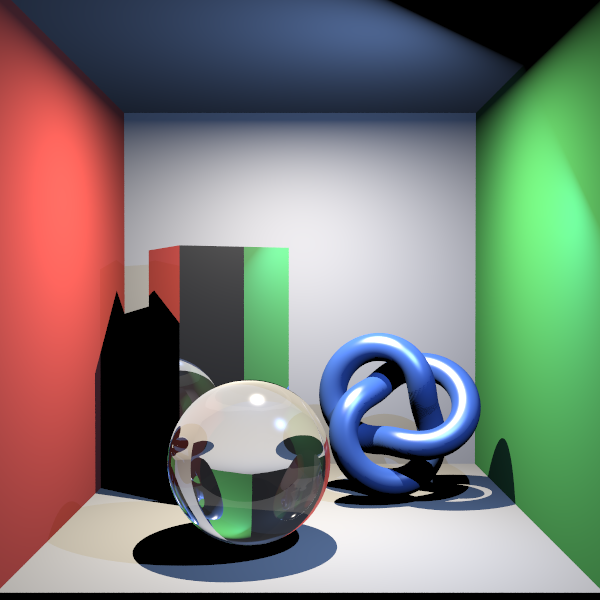
\includegraphics[width=0.78\linewidth]{room.png}
\caption{Сцена «комната»: 24\,342 треугольника, 600×600, 16 лучей на пиксель, глубина 6, нормировка на 0.2,
2 точечных ламбертовских источника (тёплый на потолке и синий справа). Зеркальный параллелепипед, стеклянная сфера
($n=1.5$), тор-узел из OBJ-файла (Блинн–Фонг), пол с бликом по Фонгу. Время 14.0 с}
\label{fig:room}
\end{figure}

\begin{figure}[H]
\centering
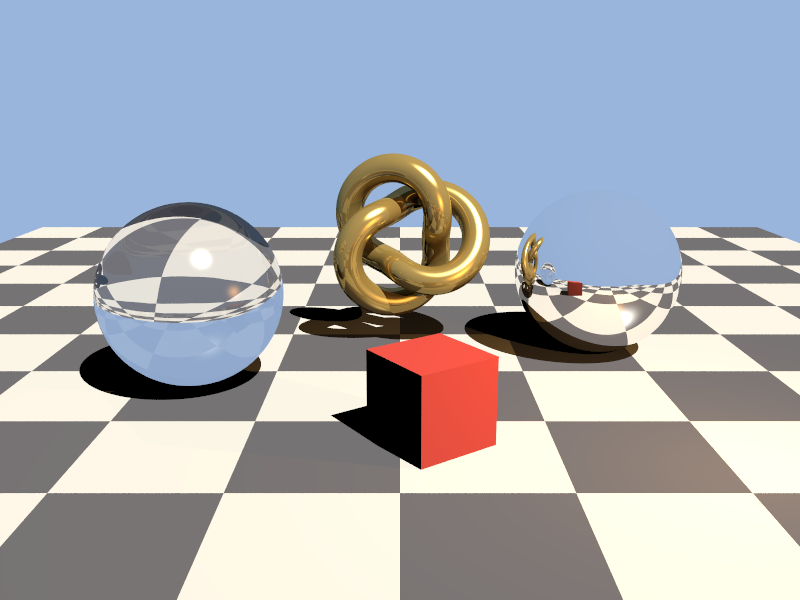
\includegraphics[width=0.85\linewidth]{outdoor.png}
\caption{Сцена «улица»: 29\,740 треугольников, 800×600, 16 лучей на пиксель. Параллельный источник (солнце) даёт
резкие тени одного направления; оранжевый точечный источник справа подсвечивает объекты тёплым светом и даёт
вторые, более слабые тени. Стеклянная сфера, зеркальная сфера, «золотой» узел
(Фонг + зеркальное отражение), пластиковый куб (Блинн–Фонг). Нормировка на среднюю яркость 0.5. Время 13.4 с}
\label{fig:outdoor}
\end{figure}

\begin{figure}[H]
\centering
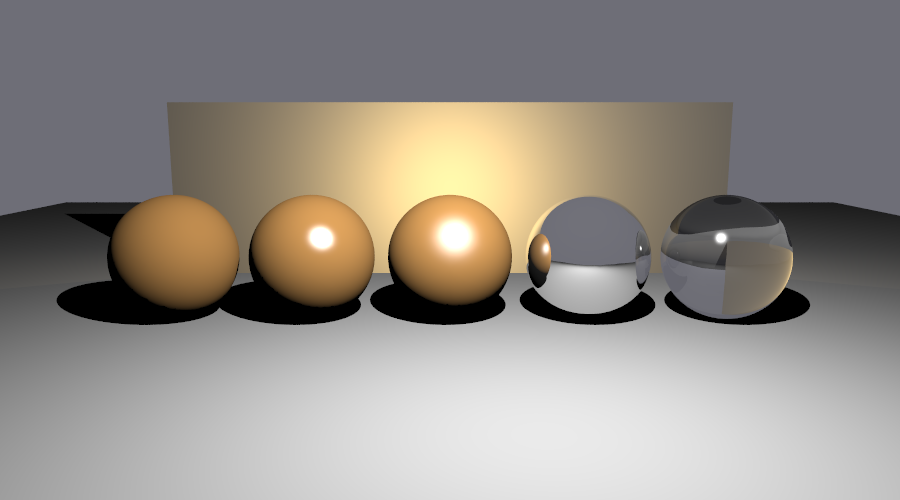
\includegraphics[width=0.95\linewidth]{materials.png}
\caption{Сравнение материалов (слева направо): Ламберт; Ламберт + Фонг ($n=30$); Ламберт + Блинн–Фонг ($n=30$);
зеркало; стекло. Сзади — экран с диффузным пропусканием $k_{dt}$, подсвеченный источником с обратной стороны.
При одинаковом $n$ блик Блинна–Фонга шире, чем у Фонга}
\label{fig:materials}
\end{figure}

\begin{figure}[H]
\centering
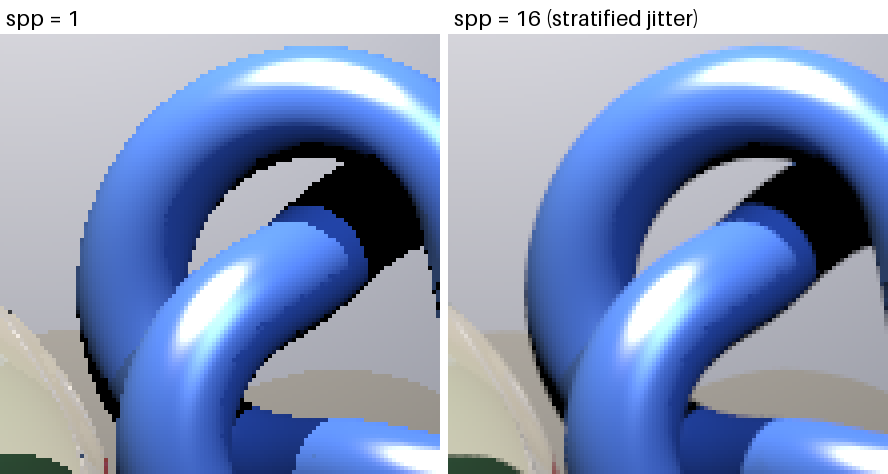
\includegraphics[width=0.9\linewidth]{aa_compare.png}
\caption{Антиалиасинг (фрагмент рис.~\ref{fig:room}, увеличение ×4): один луч через центр пикселя — ступенчатые края;
16 лучей со стратифицированным джиттером — края сглажены}
\end{figure}

\begin{figure}[H]
\centering
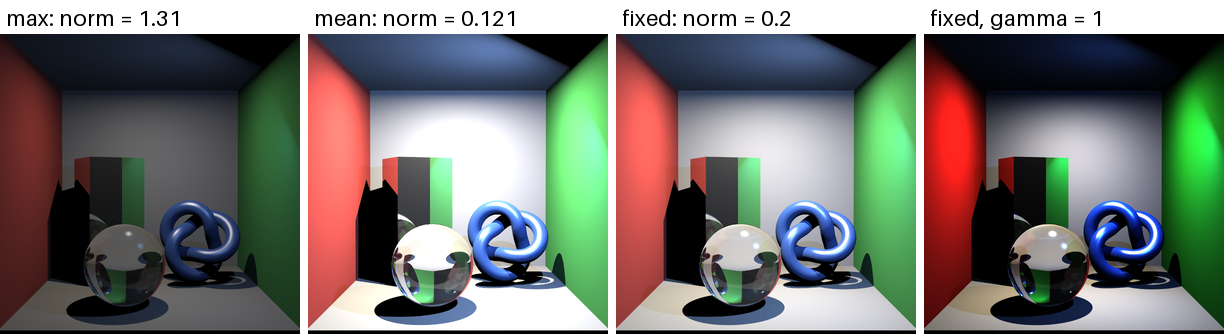
\includegraphics[width=\linewidth]{norm_compare.png}
\caption{Перевод в относительные яркости для одного и того же изображения в абсолютных яркостях:
нормировка на максимум (8.63 — яркость блика, изображение тёмное), на среднюю яркость 0.5, на заданное значение 0.2,
и то же без гамма-коррекции (тени слишком тёмные)}
\end{figure}

\begin{figure}[H]
\centering
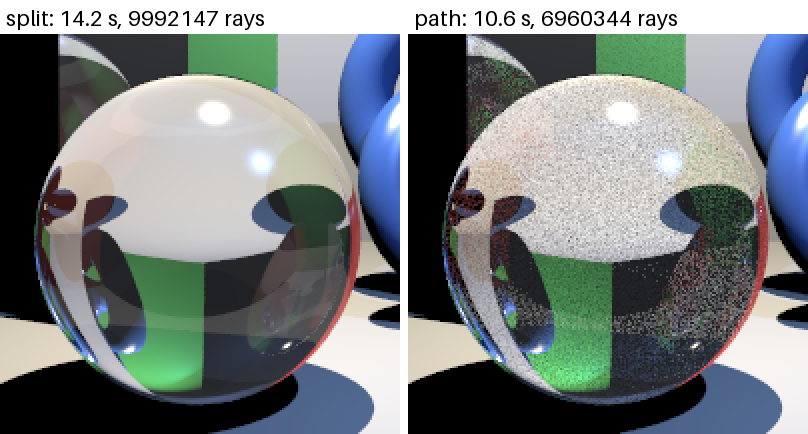
\includegraphics[width=0.9\linewidth]{mode_compare.png}
\caption{Режимы трассировки (16 лучей на пиксель): \texttt{split} — ветвление на отражённый и преломлённый лучи;
\texttt{path} — случайный выбор одного продолжения (Монте-Карло): несмещённая оценка с шумом, на 30\% меньше лучей}
\end{figure}

\section{Доказательство корректности}
\label{sec:verify}

Проверки выполняются программой \texttt{verify.py}.

\subsection{Сравнение с аналитическим расчётом яркости}

Сцена \texttt{test\_plane}: плоскость $y=0$ с $k_d=0.5$, точечный ламбертовский источник $I_0=10$ Вт/ср на высоте
$h=2$, ось направлена вниз. Для точки плоскости на расстоянии $r$ от источника $\cos\theta_s=\cos\theta=h/r$, и по
формулам (\ref{eq:point}), (\ref{eq:local}):
\begin{equation}
L = \frac{k_d}{\pi}\cdot\frac{I_0\cos\theta_s\cos\theta}{r^2} = \frac{k_d I_0 h^2}{\pi r^4}.
\end{equation}
Точка попадания луча пикселя находится независимо — пересечением луча с плоскостью $t=-o_y/d_y$:

\begin{lstlisting}
o, d = primary_rays(cam, np.array([px + 0.5]), np.array([py + 0.5]))
t = -o[0, 1] / d[0, 1]
p = o[0] + t * d[0]
r = np.linalg.norm(np.array(light["position"]) - p)
analytic = kd * i0 * h ** 2 / (np.pi * r ** 4)
traced = radiance_at(scene, backend, settings, [px + 0.5], [py + 0.5])[0, 0]
\end{lstlisting}

\begin{center}
\small
\begin{tabular}{cccccc}
\toprule
Пиксель & Точка & $r$ & $L$ аналит. & $L$ трассир. & Отн. ошибка \\
\midrule
(250, 250) & (0.007, 0, 0.009) & 2.0000 & 0.397862 & 0.397862 & $7.0\cdot10^{-16}$ \\
(250, 150) & (0.008, 0, $-$2.387) & 3.1139 & 0.0677098 & 0.0677098 & $8.2\cdot10^{-16}$ \\
(100, 250) & ($-$1.951, 0, 0.009) & 2.7939 & 0.104485 & 0.104485 & $1.3\cdot10^{-16}$ \\
(400, 400) & (1.459, 0, 2.063) & 3.2228 & 0.0590154 & 0.0590154 & $3.5\cdot10^{-16}$ \\
(120, 120) & ($-$2.414, 0, $-$3.413) & 4.6343 & 0.0138022 & 0.0138022 & $5.0\cdot10^{-16}$ \\
(480, 300) & (2.697, 0, 0.836) & 3.4598 & 0.0444277 & 0.0444277 & $1.6\cdot10^{-16}$ \\
(250, 90) & (0.010, 0, $-$4.665) & 5.0759 & 0.00959041 & 0.00959041 & $1.8\cdot10^{-16}$ \\
\bottomrule
\end{tabular}
\end{center}

Аналогично для параллельного источника ($E_0=3$, направление $(1,-2,0.5)$) и материала Ламберт ($k_d=0.5$) +
Блинн–Фонг ($k_s=0.4$, $n=20$): $L = \left(\frac{k_d}{\pi} + k_s\frac{n+8}{8\pi}(\vect n\cdot\vect h)^n\right)E_0\cos\theta$.
В четырёх точках получены значения 0.655514, 0.502620, 0.909559, 0.604621 — совпадают с аналитическими с
относительной ошибкой не более $2.2\cdot10^{-16}$. Таким образом, закон обратных квадратов, диаграмма Ламберта
источника и модели отражения реализованы верно; расхождения — на уровне машинной точности.

\subsection{Совпадение трёх способов поиска пересечений}

Для 40\,000 лучей (20\,000 первичных и 20\,000 со случайными началами и направлениями) результаты собственной BVH и Embree
сравнивались с полным перебором (заведомо правильным):

\begin{center}
\small
\begin{tabular}{llcccc}
\toprule
Сцена & Способ & Тот же треуг. & $\max|\Delta t|$ & Тени совпали & Расхожд. с равным $t$ \\
\midrule
room (24\,342) & BVH & 99.913\% & 0 & 100\% & 35 из 35 \\
room (24\,342) & Embree & 99.930\% & $8.7\cdot10^{-6}$ & 100\% & 28 из 28 \\
outdoor (29\,740) & BVH & 99.997\% & 0 & 100\% & 1 из 1 \\
outdoor (29\,740) & Embree & 100.000\% & $1.0\cdot10^{-5}$ & 100\% & 0 из 0 \\
\bottomrule
\end{tabular}
\end{center}

Все расхождения номера треугольника — лучи, у которых \emph{одинаковое} расстояние $t$ до двух треугольников
разных объектов: нижняя грань зеркального параллелепипеда лежит в плоскости пола, и оба ответа верны. Случаев
«один способ нашёл пересечение, а другой — нет» нет. Разница $t$ у Embree объясняется вычислениями в \texttt{float32}.

\subsection{Проверка теней}

Сцена \texttt{test\_shadow}: куб $0.8\times0.8\times0.8$, повёрнутый на 30\textdegree{}, на плоскости, точечный источник в
$(1.2, 2.5, 0.8)$. Для 3\,912 случайных точек плоскости независимо от треугольной сетки (пересечением отрезка
«точка — источник» с кубом в его локальной системе координат, slab-тестом) определено, находится ли точка в тени.
Результат совпал с теневыми лучами программы во всех точках:

\begin{center}
\small
\begin{tabular}{lccc}
\toprule
Способ & Точек в тени (трассировка) & Точек в тени (аналитически) & Несовпадений \\
\midrule
перебор & 204 & 204 & 0 \\
BVH & 204 & 204 & 0 \\
Embree & 204 & 204 & 0 \\
\bottomrule
\end{tabular}
\end{center}

На изображение нанесён аналитический контур тени — выпуклая оболочка проекций вершин куба из источника на плоскость
$\vect p' = \vect L + (\vect p - \vect L)\dfrac{L_y}{L_y - p_y}$ (рис.~\ref{fig:shadow}); граница тени, построенной
трассировкой, совпадает с ним.

\begin{figure}[H]
\centering
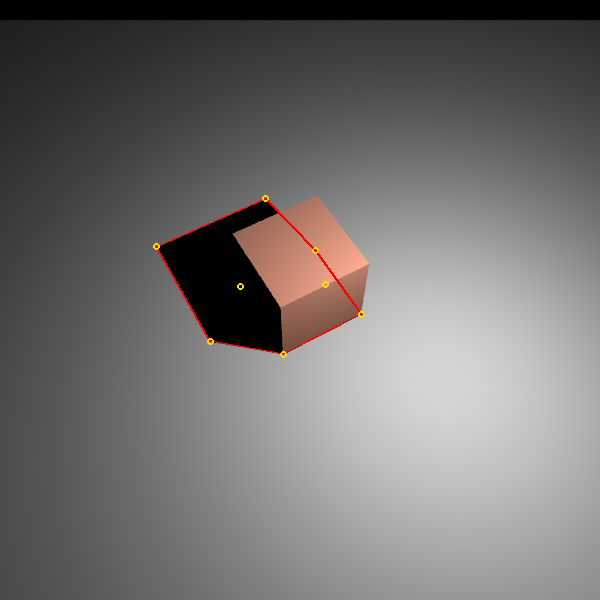
\includegraphics[width=0.55\linewidth]{verify_shadow.png}
\caption{Тень куба: красный контур — аналитическая граница тени, жёлтые точки — проекции вершин куба
(часть контура скрыта кубом от камеры)}
\label{fig:shadow}
\end{figure}

\subsection{Законы отражения и преломления}

\begin{center}
\small
\begin{tabular}{ccccc}
\toprule
$\theta_1$, \textdegree & $\theta_2$, \textdegree & $n_1\sin\theta_1$ & $n_2\sin\theta_2$ & Угол отражения, \textdegree{} \\
\midrule
0 & 0.0000 & 0.00000000 & 0.00000000 & 0.0000 \\
15 & 9.9359 & 0.25881905 & 0.25881905 & 15.0000 \\
30 & 19.4712 & 0.50000000 & 0.50000000 & 30.0000 \\
45 & 28.1255 & 0.70710678 & 0.70710678 & 45.0000 \\
60 & 35.2644 & 0.86602540 & 0.86602540 & 60.0000 \\
80 & 41.0364 & 0.98480775 & 0.98480775 & 80.0000 \\
\bottomrule
\end{tabular}
\end{center}

Закон Снеллиуса (воздух $\to$ стекло, $n=1.5$) и закон отражения выполняются. Критический угол стекло $\to$ воздух
$\arcsin(1/1.5)=41.81^\circ$: при 41.31\textdegree{} преломление есть, при 42.31\textdegree{} — полное внутреннее отражение. Для лучей,
прошедших через плоскопараллельную стеклянную пластину толщиной 0.5 (с реальным поиском пересечений), угол между
входящим и вышедшим лучами равен 0 (вышедший луч параллелен падающему), боковое смещение 0.065…0.134 при углах
падения 21…39\textdegree{} — как следует из геометрической оптики.

\subsection{Нормировка и энергия}

При нормировке \texttt{mean} средняя яркость после деления равна 0.5000, при \texttt{max} максимум равен 1.0000;
после гамма-коррекции $0.5\to186$, $0.18\to117$, $1\to255$. Сумма коэффициентов $k_d+k_s+k_r+k_t+k_{dt}$ всех
материалов во всех сценах не превышает 1 (закон сохранения энергии).

\section{Производительность}

Замеры на 12-поточном процессоре, 400\,000 первичных лучей (полный перебор — 20\,000 лучей), лучшее из трёх запусков:

\begin{center}
\small
\begin{tabular}{lrlrrr}
\toprule
Сцена & Треуг. & Способ & Построение, с & Узлов / глубина & Млн лучей/с \\
\midrule
room & 24\,342 & перебор (12 потоков) & — & — & 0.057 \\
room & 24\,342 & BVH (1 поток) & 0.960 & 15\,117 / 17 & 4.71 \\
room & 24\,342 & BVH (12 потоков) & 0.989 & 15\,117 / 17 & 32.50 \\
room & 24\,342 & Embree (1 поток) & 0.026 & — & 8.71 \\
\midrule
outdoor & 29\,740 & перебор (12 потоков) & — & — & 0.045 \\
outdoor & 29\,740 & BVH (1 поток) & 1.230 & 18\,603 / 18 & 4.59 \\
outdoor & 29\,740 & BVH (12 потоков) & 1.241 & 18\,603 / 18 & 24.87 \\
outdoor & 29\,740 & Embree (1 поток) & 0.028 & — & 9.19 \\
\midrule
materials & 26\,114 & перебор (12 потоков) & — & — & 0.052 \\
materials & 26\,114 & BVH (1 поток) & 1.065 & 16\,807 / 17 & 4.73 \\
materials & 26\,114 & Embree (1 поток) & 0.025 & — & 9.61 \\
\bottomrule
\end{tabular}
\end{center}

Собственная BVH ускоряет поиск пересечений по сравнению с полным перебором при одинаковом числе потоков (12)
в 500–570 раз; даже однопоточная BVH примерно в 80 раз быстрее 12-поточного перебора. Embree в одном потоке ещё примерно в 2 раза быстрее нашей BVH и строит структуру почти в
40 раз быстрее (оптимизированный C++ и SIMD). Обёртка \texttt{embreex} вызывает Embree для лучей последовательно в
одном потоке, поэтому многопоточная BVH на \texttt{numba} в этом окружении обгоняет её. Полное время рендера
сцены «комната» 600×600×4 луча: 3.46 с с BVH и 3.72 с с Embree — основное время занимает расчёт освещения.

\section*{Выводы}
\addcontentsline{toc}{section}{Выводы}

В работе реализован синтез изображений трёхмерных сцен методом обратной трассировки путей с локальным освещением.
Геометрия сцены задаётся треугольной сеткой (в том числе импортируемой из OBJ-файла); пересечение луча с
треугольником вычисляется алгоритмом Мёллера–Трумбора. Для ускорения реализована ускоряющая структура BVH,
построенная по эвристике площади поверхности, а также подключена готовая библиотека трассировки Intel Embree;
способы поиска пересечений взаимозаменяемы. Учтены модели Ламберта, Фонга и Блинна–Фонга, идеальное зеркальное
отражение, преломление по закону Снеллиуса с полным внутренним отражением и диффузное пропускание; источники —
точечные с диаграммой Ламберта и параллельные, цветные; тени строятся теневыми лучами. Изображение формируется в
абсолютных яркостях и переводится в относительные с нормировкой, отсечением и гамма-коррекцией, записывается в PPM;
используется стратифицированный антиалиасинг.

Корректность доказана: рассчитанные яркости совпадают с аналитическими с точностью до машинной погрешности
($<10^{-15}$); собственная BVH и Embree дают те же пересечения, что и полный перебор (все расхождения — равноудалённые
совпадающие грани); тени совпадают с независимой аналитической проверкой во всех 3\,912 точках; законы отражения и
преломления выполняются. Ускоряющая структура сокращает число проверок с десятков тысяч треугольников до ~10 узлов
дерева на луч и ускоряет поиск пересечений в 500–570 раз по сравнению с полным перебором.

\newpage
\appendix
\section*{Приложение. Исходный код программы}
\addcontentsline{toc}{section}{Приложение. Исходный код программы}

\subsection*{main.py}
\lstinputlisting{code/main.py}
\subsection*{scene.py}
\lstinputlisting{code/scene.py}
\subsection*{accel.py}
\lstinputlisting{code/accel.py}
\subsection*{render.py}
\lstinputlisting{code/render.py}
\subsection*{verify.py}
\lstinputlisting{code/verify.py}

\end{document}
